\documentclass[25pt, a0paper,
               colspace=15mm, subcolspace=0mm,
               blockverticalspace=17mm]{tikzposter} % See Section 

\usepackage{poster}
\usepackage{array}
\usepackage{multirow}
\usepackage{multicol}


\definecolor{PaleBlue}{rgb}{0,.55,.9}
\definecolor{PaleGreen}{rgb}{0,.7,.25}
\definecolor{RedPink}{rgb}{.9,0,.2}
\definecolor{Pink}{rgb}{.85,.35,.7}
\definecolor{Purple}{rgb}{.6,0,.75}
\definecolor{Orange}{rgb}{.9,.3,.05}

\colorlet{attentionColor}{Orange}
\colorlet{charEmbedColor}{RedPink}
\colorlet{predEmbedColor}{Pink}
% \colorlet{attentionColor}{GoldUL!90!black}
% \definecolor{attentionColor}{rgb}{.85,.5,.6}



\def\pathwidth{2pt}
\def\nodewidth{3pt}
\def\cornerCurvature{7pt}

\tikzstyle{embed}=[%
  draw,
  #1,
  % line width=3pt,
  anchor=north,
  minimum width=.8cm,
  minimum height=1.6cm,
  inner sep=0pt,
  text=#1!65!black,
  font=\fontsize{25pt}{24}\selectfont,
  ]




\title{\parbox{\linewidth}{\centering Pruning Filters In Convolution Neural Network}}
\institute{Department of Computer Science and Software Engineering, Université Laval}
\author{Vincent Martineau}

\begin{document}
\maketitle

\begin{columns}
\column{.4}
\block{Introduction}{%
We explore how reducing network expressivity can affect performance in Convolution Neural Network (CNN). We implemented a pruner that can remove filters from convolution layer and explore the effect on transfer learning tasks. 

\vspace{5mm}
\textbf{Motivations:}
\begin{itemize}
  \item \colorbold{Reduce} network size.
  % \item Goldberg (2017) emphasizes this fact for NLP tasks such as part of speech tagging (POS) or named entity recognition (NER).
  \item \colorbold{Improve} execution speed.
\end{itemize}

\vspace{5mm}
\textbf{Related work:}
\begin{itemize}
  \item P.Molchanov et al. (2017): Pruning Convolutional Neural Networks for Resource Efficient Inference.
\end{itemize}

\vspace{0mm}
\textbf{Goals:}
\begin{itemize}
  \item Evaluate the impact of reducing network expression on performance.
  \item Compare training time on various model.
  \item Compare various strategies to prune.
  \item Provide a module that could.
\end{itemize}

% \vspace{-15pt}

}

\column{0.6}
\block{Comparing Various level of Pruning in AlexNet}{

\vspace{-15pt}
% Comick v3.0 (TheFinalComick)
\begin{center}
	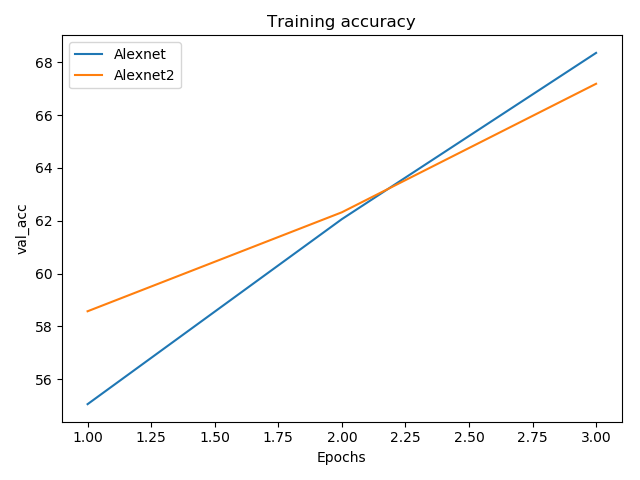
\includegraphics{figures/prune_ratio}
\end{center}

The net consists in 3 bi-LSTM taking as input the left context, the right context and the word characters. An attention module ponderates their outputs which are then combined in a last fully connected layer.

}
\end{columns}

\begin{columns}
\column{.6}


% \block[bodyoffsety=48mm, titleoffsety=48mm]{Experiments}{
\block{Experiments}{

\textbf{Set up:}
\begin{itemize}
  \item Labeling tasks:
  \begin{itemize}
      \item \colorbold{Named Entity Recognition} (NER).
      \item \colorbold{POS tagging} (POS).
  \end{itemize}
  \item Dataset: \colorbold{CoNLL 2003}
  
%   \item Two nets working together:
%   \begin{itemize}
%     \item One predicts OOV embeddings (see OOV handling net section).
%     \item One predicts tags (see Labeling task section).
%   \end{itemize}
  % \item Baseline: randomly generated embeddings for OOV.
\end{itemize}


\textbf{Training details:}
\begin{itemize}
    \item Tensors sizes:
    \begin{itemize}
        \item Char. emb.: 20.
        \item Word emb.: 100 (\colorbold{GloVe}).
        \item LSTMs hidden state: 128.
    \end{itemize}
    \item Context size from 2 words to the whole sentence.
    \item Standard learning rate on the labeling task parameters, reduced learning rate on Comick using SGD (0.01, 0.001).
\end{itemize}


% \textbf{Experiments:}
% \begin{itemize}
%   \item Performance gains:
%   \begin{itemize}
%     \item Comparison between accuracies for POS.
%     \item Comparison between F1 scores for NER.
%   \end{itemize}
%   \item Interpretability:
%   \begin{itemize}
%     \item Comparison of the average weights given to the left context, right context and the words by the network by tags.
%     \item Qualitative examples of where we observe a shift of attention according to the context.
%   \end{itemize}
% \end{itemize}

\vspace{-.25mm}

}


  \column{.38}
  \block[bodyoffsety=0mm, titleoffsety=0mm]{Examples}{
  \vspace{-2mm}
  \begin{center}
  \Large
  % \resizebox{\textwidth}{!}{%
  \setlength{\tabcolsep}{8pt}
  \begin{tabular}{c c c c c c c c}
  \toprule
  \multirow{2}{*}{\textbf{Entity}} & \multicolumn{3}{c}{\textbf{Ponderation}} & \multirow{2}{*}{\textbf{Examples}}\\
  \cline{2-4}
  \addlinespace[2mm]
  & Word & Left & Right & \\
  \midrule
  \texttt{PER} & 0.19 &  \colorbold{0.49} & 0.32 & \textbf{in sentencing darrel} \underline{\textit{voeks}} , 38 , to a 10-year prison term on thursday\\
  \texttt{PER} & 0.15 &  \colorbold{0.59} & 0.26 &   \textbf{\texttt{<BOS>} australian parliamentarian john} \underline{\textit{langmore}} has formally resigned from his lower house\\
  \texttt{PER} & 0.15 &  \colorbold{0.61} & 0.24 &  had received today \textbf{from mr john vance} \underline{\textit{langmore}} , a letter resigning his place as \\
  \texttt{PER} & 0.15 &  \colorbold{0.69} & 0.16 &  \textbf{\texttt{<BOS>} rtrs - australian mp john} \underline{\textit{langmore}} formally resigns . \texttt{<EOS>}\\
  \texttt{ORG} & 0.22 & \colorbold{0.46} & 0.32 &  the number of plastic surgeries in [...] the \textbf{brazilian plastic surgery society} ( \underline{\textit{sbcp}} ) , said ,\\
  \texttt{ORG} & 0.28 & 0.23 & \colorbold{0.49} &  to increase them in the united states , " \underline{\textit{sbcp}} \textbf{vice-president oswaldo saldanha said}\\
  \texttt{LOC} & 0.16 & 0.22 & \colorbold{0.62} &  some residents of the \underline{\textit{kazanluk}} \textbf{area are moslems who} converted to islam during \\
  \texttt{LOC} & 0.20 & \colorbold{0.47} & 0.33 &  at a mosque in the \textbf{central bulgarian town of} \underline{\textit{kazanluk}} , causing damage but no injuries\\
  \texttt{MISC} & \colorbold{0.68} & 0.11 & 0.21 &  freestyle \textbf{\underline{\textit{skiing-world}}} cup aerials results .\\
  \texttt{MISC} & \colorbold{0.42} & 0.18 & \colorbold{0.40} & the \textbf{\underline{\textit{franco-african}} summit decided to send} a mission bangui [...] civil war .\\
  %0.17 &  0.40 & \colorbold{0.43} &   \textbf{\texttt{<BOS>}} \textit{langmore} \textbf{, 57 , announced in november that}\\
  \bottomrule
  \end{tabular}
  \end{center}
  
  \vspace{2mm}
  Qualitative example on several OOV words (underlined). We can see that depending on the context and the target, the weights may shift drastically.
  % \vspace{5.5mm}
  }
  




\end{columns}




















\begin{columns}

  \column{.3}


  \block{Labeling task net}{

  \begin{center}
  \begin{tikzpicture}[
          scale=1.5,
          lstm_right/.style={draw, minimum width=1cm, minimum height=.5cm, inner sep=0pt, anchor=north, PaleGreen},
          lstm_left/.style={draw, minimum width=1cm, minimum height=.5cm, inner sep=0pt, PaleBlue},
          every path/.style={line width=\pathwidth},
          every node/.append style={line width=\nodewidth}]
    \def\h{2cm}
    \def\scalespace{2.2}
    \def\w{145mm}
    \def\arrowLen{.6}
    \def\descSpace{-.2}

    % Char embedding

    \foreach \word/\color/\w [count=\i] in {Salem/gray/o, Bitar/gray/o, appeared/Purple/w, to/Purple/w, have/Purple/w}{
      \pgfmathsetmacro\pos{\i-1}
      \node[anchor=mid, inner sep=0](\word) at (\scalespace*\pos,0) {\word};
      \node[embed=\color,draw=\color](\word _embed) at (\scalespace*\pos,-\arrowLen){\w};
    };

    \node[embed=black, minimum width=\w, minimum height=\h, anchor=north](comick) at ([yshift=-\arrowLen cm]appeared_embed.south) {OOV handling net};
    % \node[anchor=east, align=left] at ([xshift=\descSpace cm]comick.west) {OOV \\ handling};

    \foreach \word/\color/\w [count=\i] in {Salem/predEmbedColor/p, Bitar/predEmbedColor/p, appeared/Purple/w, to/Purple/w, have/Purple/w}{
      \pgfmathsetmacro\pos{\i-1}

      \path (\word _embed) edge[draw, -mytip] (comick.north -| \word _embed.south);
      \draw[-mytip] (comick.south -| \word _embed) -- ++(0,-\arrowLen) node[anchor=north, embed=\color, draw=\color](\word _pred_embed) {\w};

      \node[lstm_left, draw=PaleBlue, anchor=north](\word _lstm_left) at ([yshift=-\arrowLen cm]\word _pred_embed.south) {};
      \node[lstm_right, draw=PaleGreen](\word _lstm_right) at (\word _lstm_left.south) {};
      \draw[-mytip] (\word _pred_embed) -- (\word _lstm_left);
  
    };

    % LSTM arrows
    \foreach \a/\b in {Salem/Bitar, Bitar/appeared, appeared/to, to/have}{
      \draw[mytip-, PaleBlue] (\a _lstm_left) -- (\b _lstm_left);
      \draw[-mytip, PaleGreen] (\a _lstm_right) -- (\b _lstm_right);
    };
    % \node[anchor=east, align=left] at ([xshift=\descSpace cm]Salem_lstm_left.south west) {Bi-LSTM \\ task net};


    \foreach \word/\tag [count=\i] in {Salem/B-PER, Bitar/I-PER, appeared/O, to/O, have/O}{
      \pgfmathsetmacro\pos{\i-1}

      \draw[-mytip] (\word  _lstm_right.south) -- ++(0,-\arrowLen) node[embed=Orange](\word _softmax) {s};

      \node[anchor=mid, inner sep=0] (\word _tag) at ([yshift=-.5cm]\word _softmax.south) {\tag};
    };
    % \node[anchor=east, align=right] at ([xshift=\descSpace cm]Salem_tag.west) {Tags};


    % Legend
    % \begin{scope}[xshift=10.7cm, yshift=-2cm,
    \begin{scope}[xshift=-15mm, yshift=-105mm,
            every path/.style={line width=\pathwidth},
            every node/.append style={line width=\nodewidth}]
    \def\legspace{-1.3}
    \def\colsep{7}
    \def\h{1.3cm}
    % First col
    \node[embed=gray, anchor=center, minimum height=\h, minimum width=.8cm](leg char embed) at (0,0*\legspace) {o};
    \node[anchor=west] at (.5,0*\legspace) {OOV word embedding};

    \node[embed=Purple, anchor=center, minimum height=\h, minimum width=.8cm](leg word embed) at (0,1*\legspace) {w};
    \node[anchor=west] at (.5,1*\legspace) {Word embedding};

    \node[embed=predEmbedColor, anchor=center, minimum height=\h, minimum width=.8cm](leg word embed) at (0,2*\legspace) {p};
    \node[anchor=west, align=left] at (.5,2*\legspace) {Predicted embedding};


    \node[draw, PaleBlue, minimum width=1cm, inner sep=0pt, minimum height=.5cm, anchor=south] (leg lstm left) at (\colsep,0*\legspace) {};
    \node[draw, PaleGreen, minimum width=1cm, inner sep=0pt, minimum height=.5cm, anchor=north] (leg lstm right) at (leg lstm left.south) {};
    \node[anchor=west] at (\colsep+.5,0*\legspace) {Bidirectional LSTM};

    \node[embed=Orange, anchor=center, minimum height=\h, minimum width=.8cm](leg word embed) at (\colsep,1*\legspace) {s};
    \node[anchor=west, align=left] at (\colsep+.5,1*\legspace) {Tag prediction\\ with a softmax};

    \end{scope}


  \end{tikzpicture}
  \end{center}
  % \vspace{3mm}

  Two nets working together: the first predicts OOV embeddings (see OOV handling net section) and the second one predicts tags.

  The simple architecture of the labeling net is used to emphasize the usefulness of our module, and to minimize the influence of other factors.

  \vspace{-.5mm}

  }









  \column{.3}
  \block{Interpretability}
  {
  \begin{center}
  \setlength{\tabcolsep}{5mm}
  \begin{tabular}{c c c c c c}
  \toprule
  \multirow{2}{*}{\textbf{Task}} & \multirow{2}{*}{\textbf{Tag}} & \multirow{2}{*}{\textbf{Ex.}} & \multicolumn{3}{c}{\textbf{Ponderation}}\\
  \cline{4-6}
  \addlinespace[3mm]
  & & & Word & Left & Right\\
  \midrule
  \multirow{9}{*}{NER} & O           & 1039  & \colorbold{0.81}    & 0.08    & 0.11 \\
  & B-PERS      & 63    & 0.21    & 0.31    & \colorbold{0.49} \\
  & I-PER     & 119   & 0.16  & \colorbold{0.52} & 0.32 \\
  & B-ORG     & 40  & 0.26  & 0.30  & \colorbold{0.44} \\ 
  & I-ORG     & 3     & 0.27  & 0.31      & \colorbold{0.42} \\
  & B-LOC     & 13  & 0.23      & 0.30  & \colorbold{0.47} \\
  & I-LOC     & 2     & 0.16  & \colorbold{0.48} & 0.36 \\
  & B-MISC      & 47  & \colorbold{0.40} & 0.21  & 0.39 \\
  & I-MISC      & 5     & \colorbold{0.41} & 0.26  & 0.33 \\
  \midrule
  \multirow{5}{*}{POS} & NNP  & 308 & 0.29  & 0.31  & \colorbold{0.40} \\
  & NN  & 46  & \colorbold{0.45} & 0.20  & 0.35 \\
  & CD  & 827 & \colorbold{0.86} & 0.05  & 0.09 \\
  & NNS & 23  & \colorbold{0.37} & 0.24  & \colorbold{0.39} \\
  & JJ  & 100 & \colorbold{0.49} & 0.15  & 0.36 \\
  \bottomrule
  \end{tabular}
  \end{center}
  
  \vspace{1.5mm}
   Average weights assigned to word's characters, left context and right context by the attention mechanism. We can clearly see the shift of attention according to the target entity. We also observe that the attention depends on the task at hand.
  \vspace{-3mm}
  }







  
  
  
  \column{.4}
  

  \block{Performance gain}{%
  \begin{center}
  \setlength{\tabcolsep}{5mm}
  \begin{tabular}{c c c c c}
  \toprule
  \textbf{Task} & \textbf{Metric} & \textbf{Random Emb.} & \textbf{Our module} & \textbf{Gain}\\
  \midrule
  NER      & F1   & 77.56 & \colorbold{80.62} & 3.9\% \\
  POS      & acc. & 91.41 & \colorbold{92.58} & 1.2\% \\
  % Chunking & acc. & 92.63 & 93.16  & \textbf{93.19} \\
  % Keyphrase& F1   & 37.40 & 39.56 & \textbf{39.77} \\
  \bottomrule
  \end{tabular}
  \end{center}
  
  \vspace{2.5mm}
  The impact of our model on two NLP downstream tasks. We compare our OOV embeddings prediction scheme against random embeddings.
  \vspace{-12mm}
  }


  
  
  
  
  
  
  
  
  
  
  
  
  \block{Conclusion}{
  
  \textbf{Discussion:}
    \begin{itemize}
        \item \colorbold{Morphology} and \colorbold{context} help predict useful embeddings.
        \item \colorbold{The attention mechanism works}: depending on the task, the network will use either more the context or the morphology to generate an embedding.
    \end{itemize}
    
    \textbf{Future works:}
    \begin{itemize}
        \item  Apply the \colorbold{attention mechanism on each character of the OOV word and each word of the context} instead of using the hidden state of the respective elements only.
        \item Test our attention model in \colorbold{different languages} and on other NLP tasks, such as \colorbold{machine translation}.
    \end{itemize}
    \vspace{-3.5mm}
  }
\end{columns}

\end{document}
